%!TEX root = ../prace.tex

\section{Kyselý déšť}

Pokud se blíží bouře kyselého deště, nebo právě jedna probíhá, hráč vidí v levé horní části obrazovky zprávu s odhadovaným časem a intenzitou.

To umožňuje strategicky řídit chod svých budov a případně limitovat spotřebovávané zdroje v případě očekávaných dlouhotrvajících bouří. Odhadovaný čas je udán v herním čase.

\begin{figure}[!h]\centering
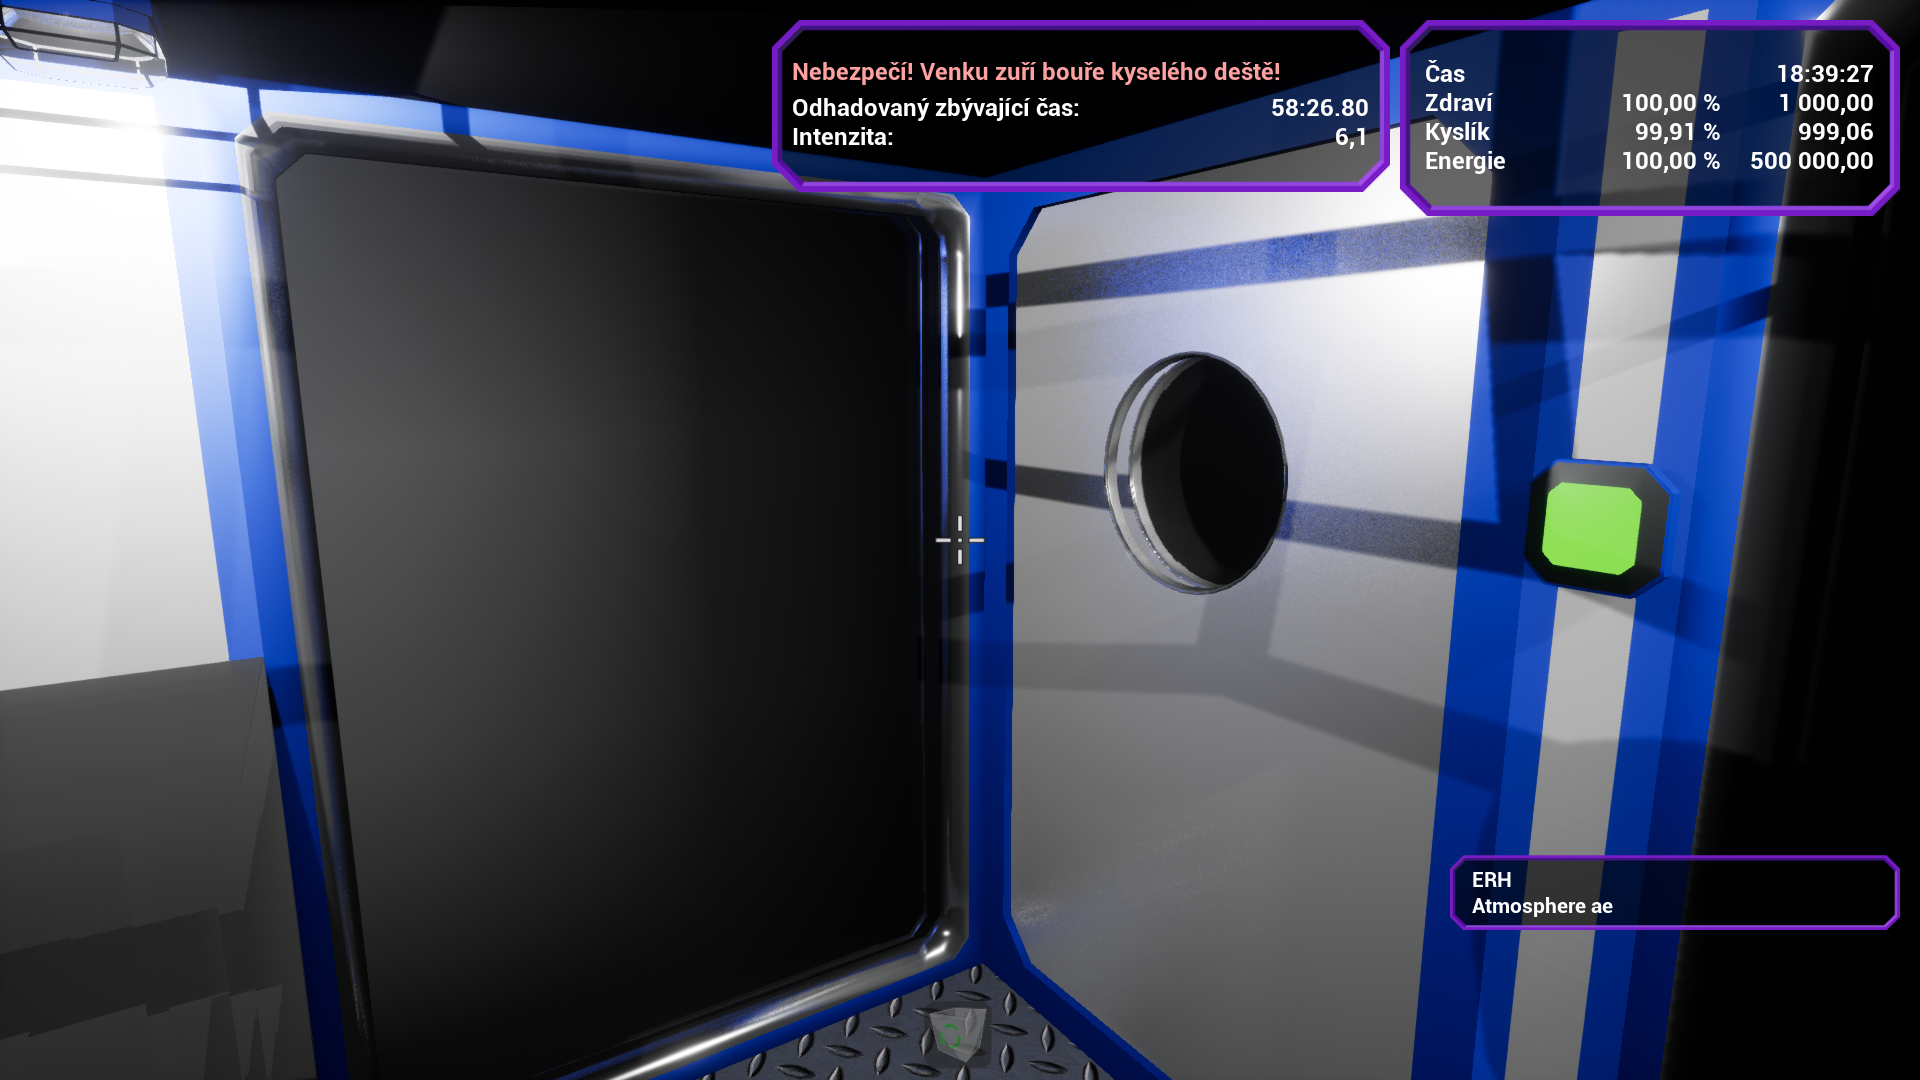
\includegraphics[ width=140mm]{../img/user/rain/0rainInfo}

\caption{Kyselý déšť - info}
\label{fig:user_rain_0rainInfo}

\end{figure}

\FloatBarrier

Pokud hráč není ukrytý v budově či pod nějakým blokem, dostává zásahy. Dokud má dostatek energie, je schopen odolávat účinkům bouře, v momentě, kdy mu energie dojde, začne mu ubývat zdraví.


\begin{figure}[!h]\centering
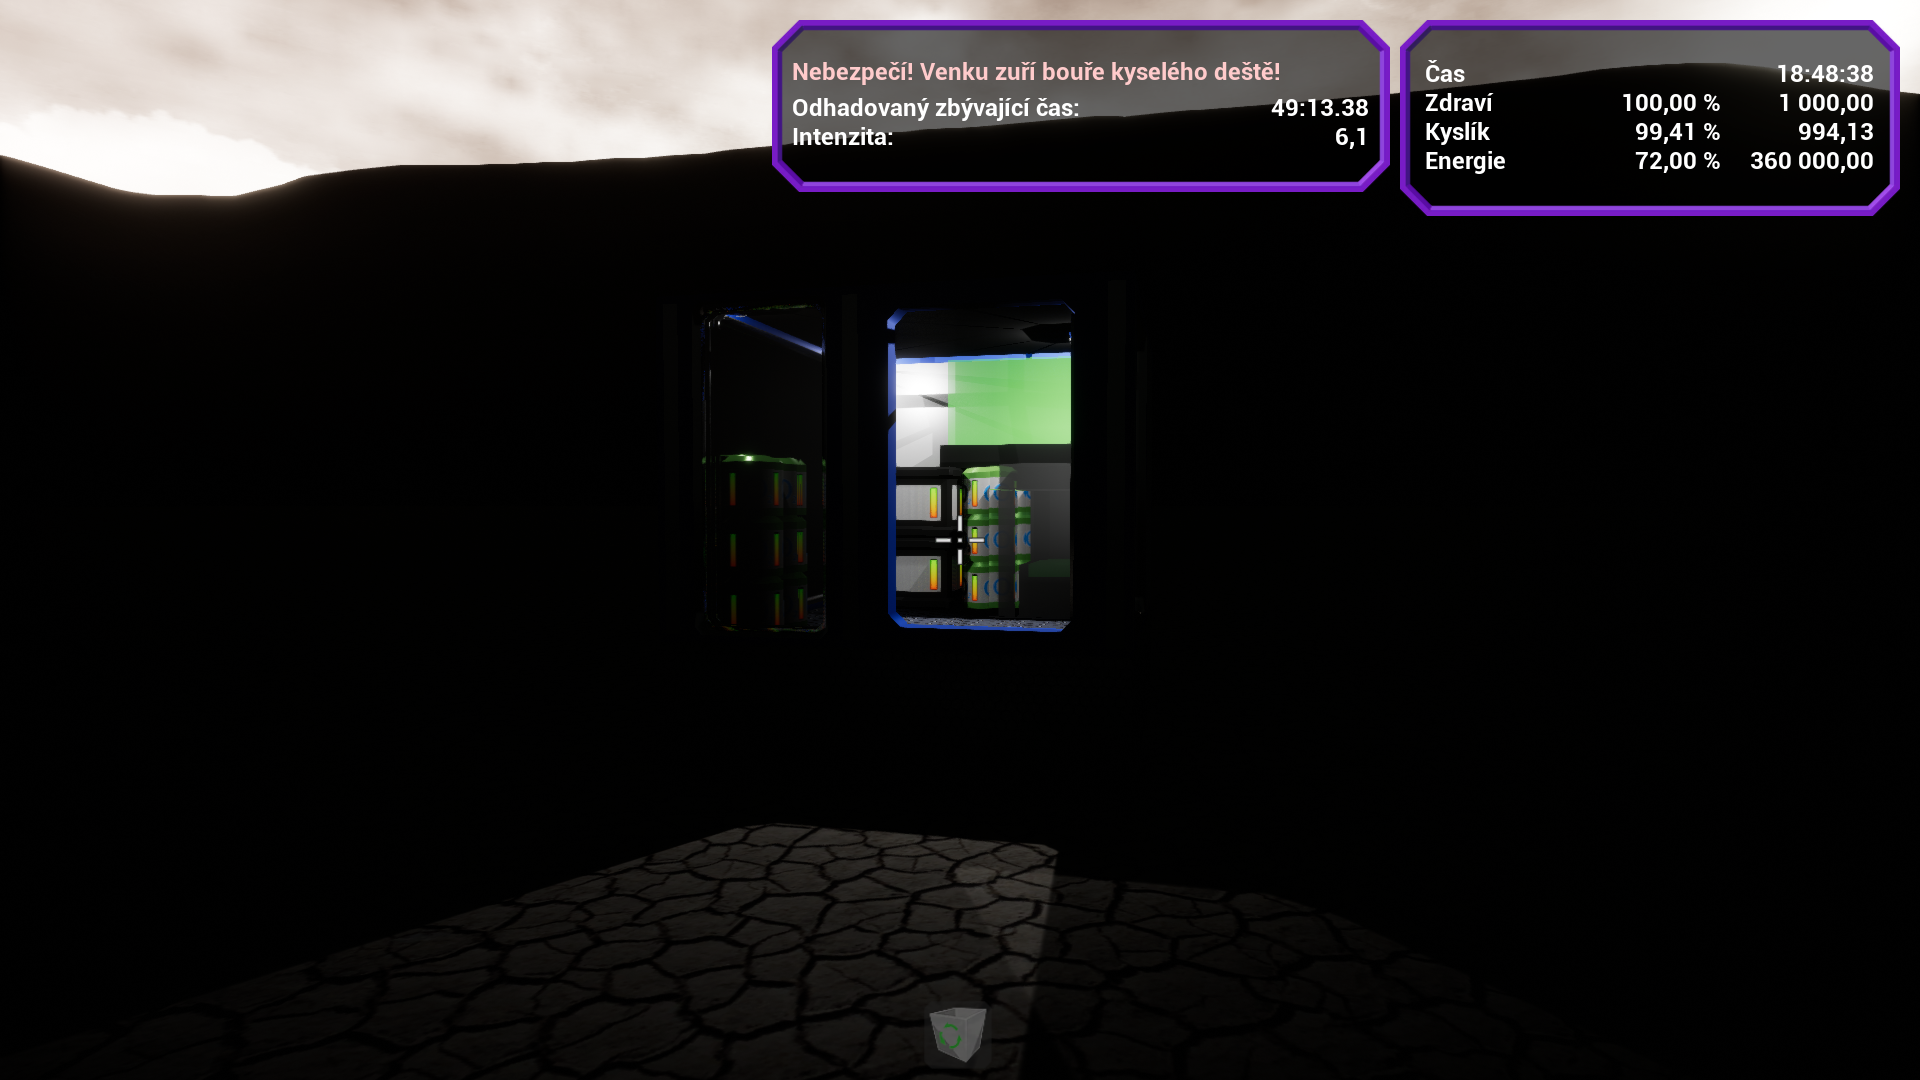
\includegraphics[ width=140mm]{../img/user/rain/1rainDamage}

\caption{Kyselý déšť - zásahy}
\label{fig:user_rain_1rainDamage}

\end{figure}

\FloatBarrier

Pokud si hráč doplní energii, začne se mu zdraví obnovovat.

\begin{figure}[!h]\centering
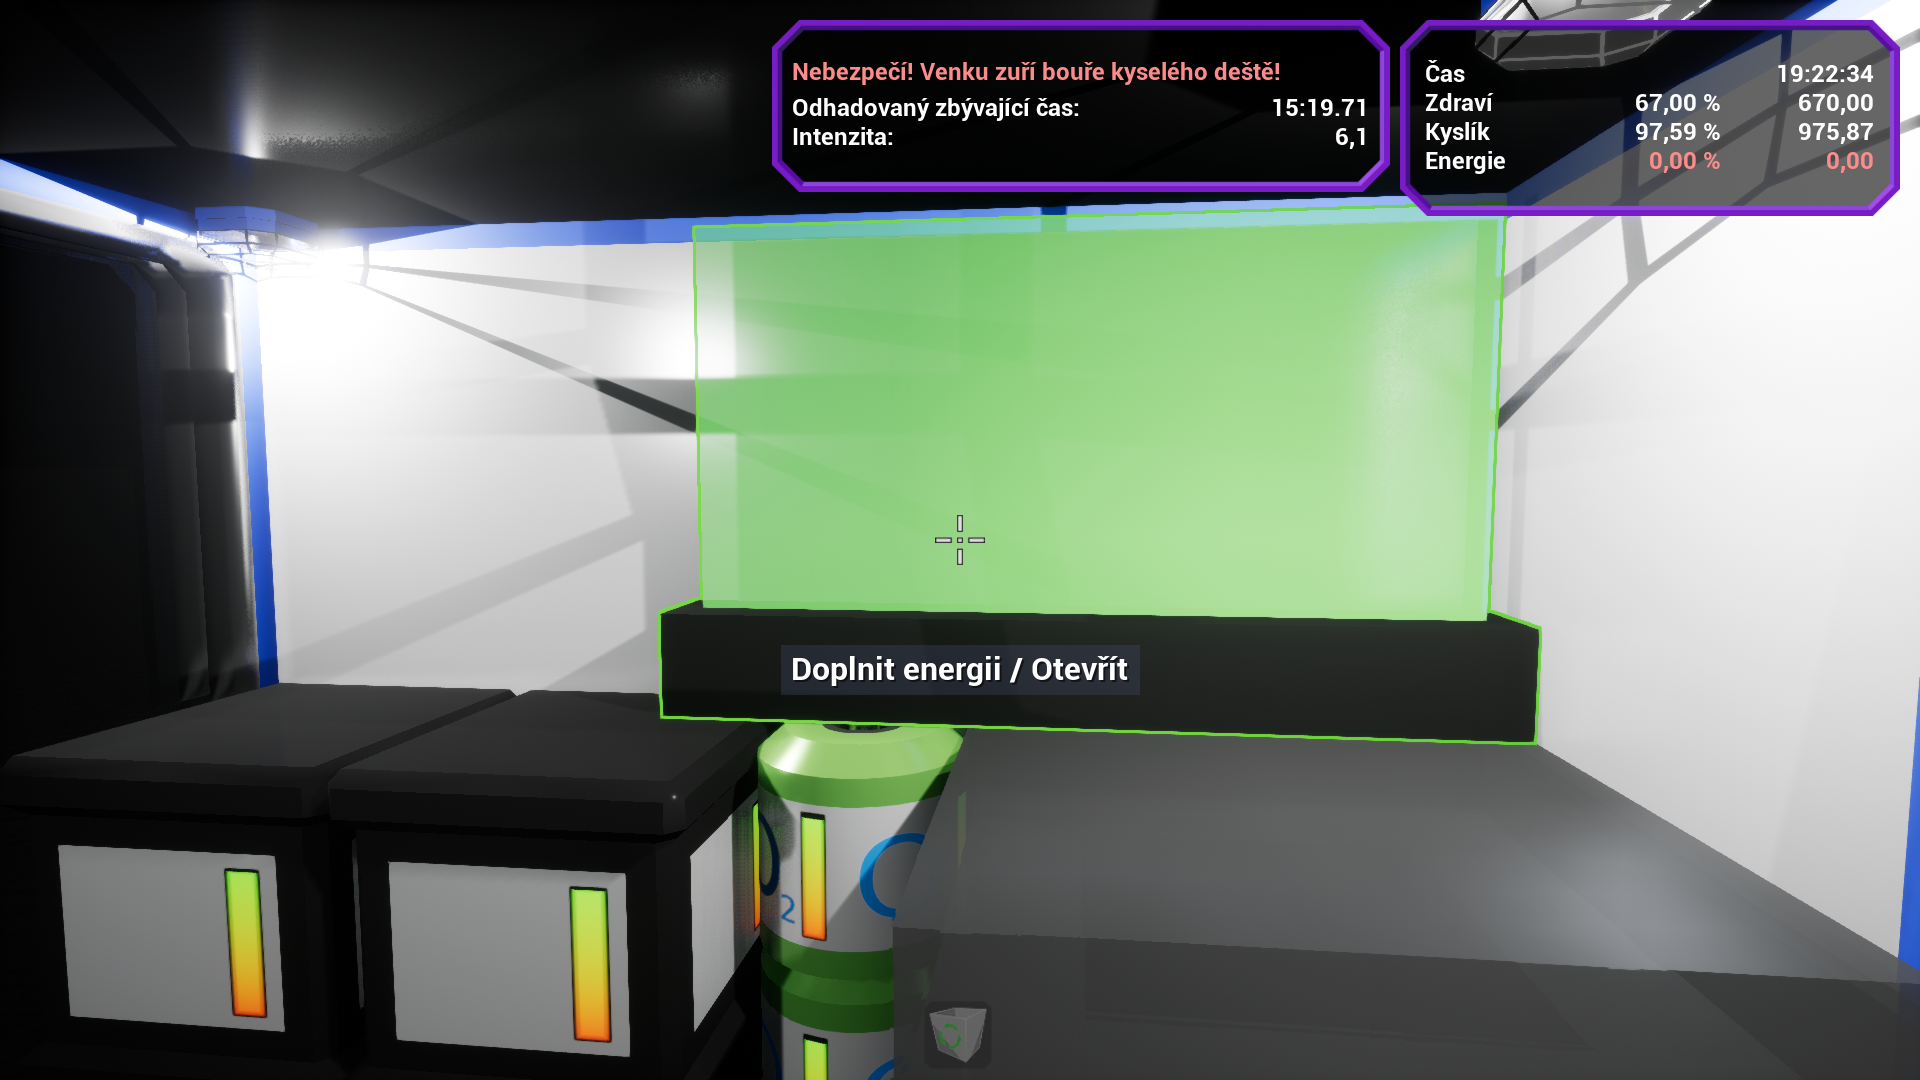
\includegraphics[ width=140mm]{../img/user/rain/2rainRefill}

\caption{Kyselý déšť - obnova zdraví}
\label{fig:user_rain_2rainRefill}

\end{figure}


\begin{figure}[!h]\centering
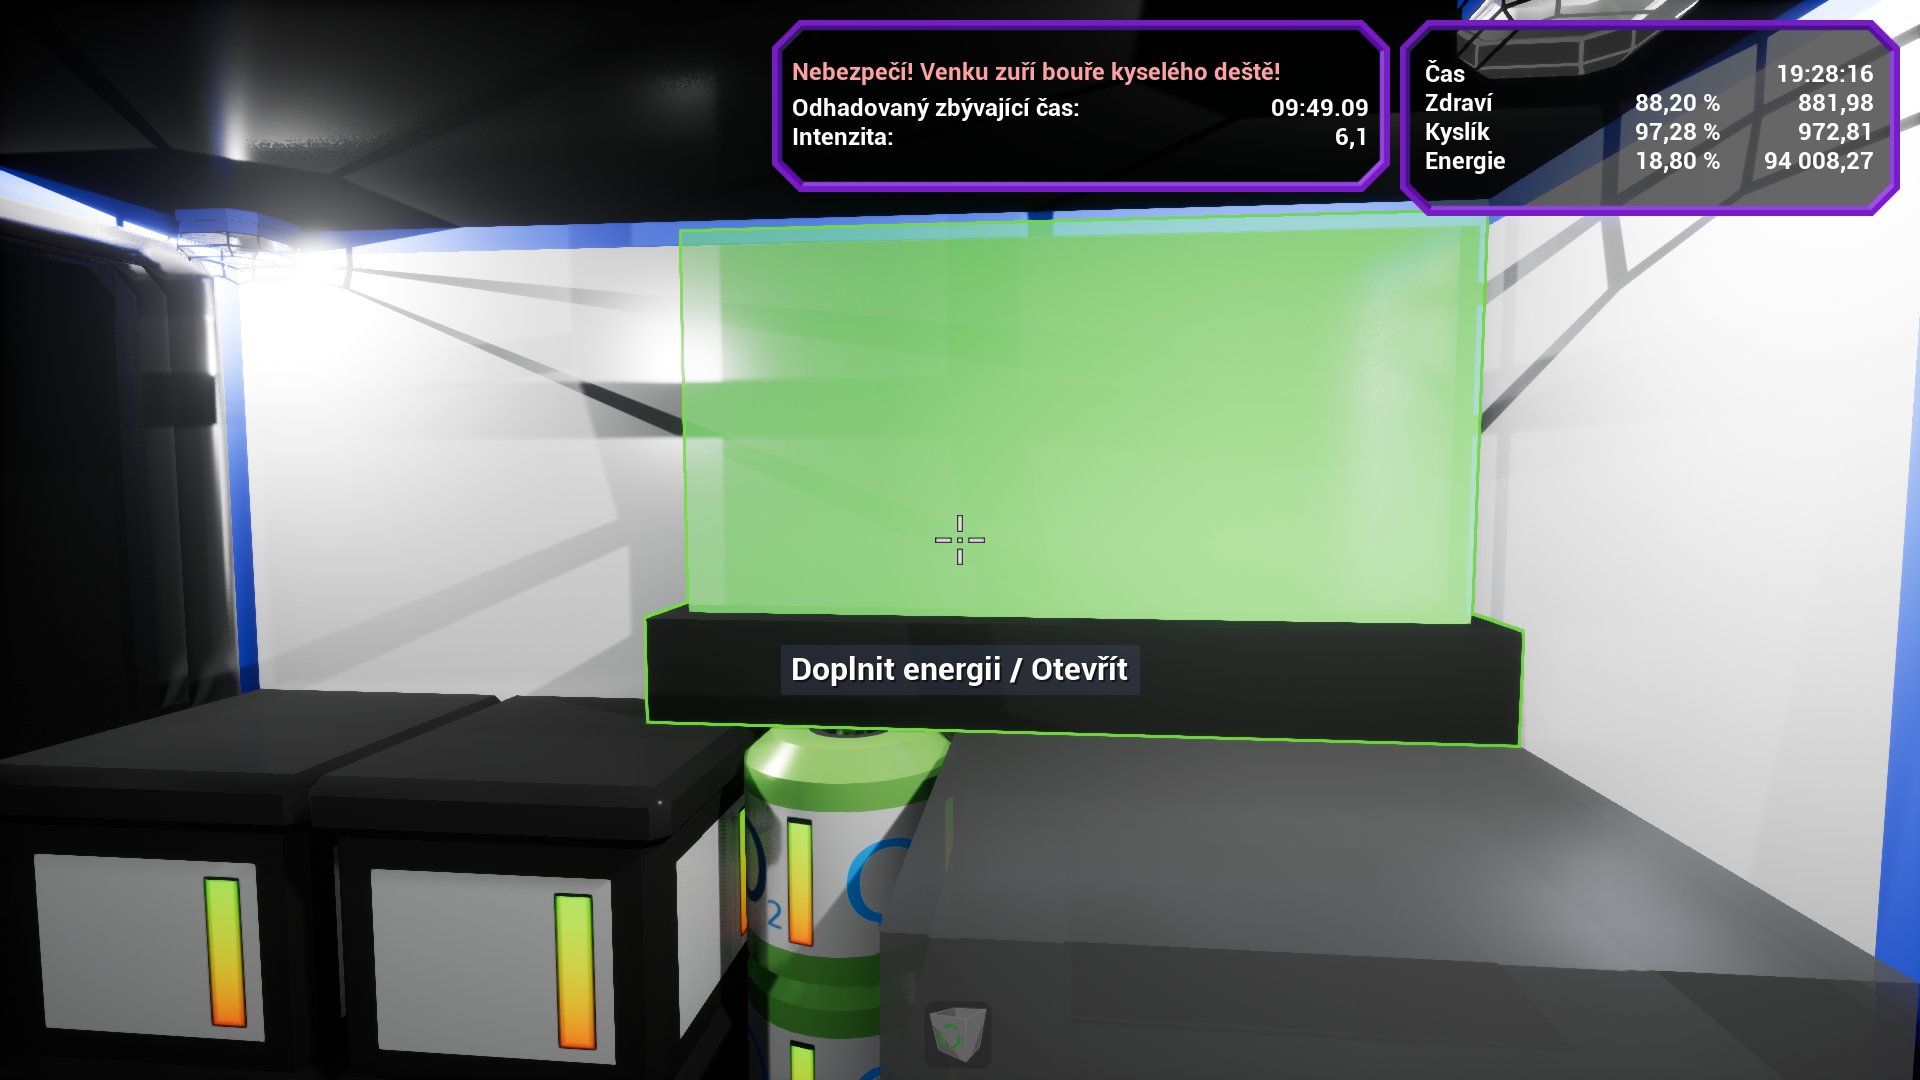
\includegraphics[ width=140mm]{../img/user/rain/3rainRefill1}

\caption{Kyselý déšť - obnova zdraví}
\label{fig:user_rain_3rainRefill1}

\end{figure}

\FloatBarrier

Během bouře je též možné pozorovat animaci generátoru energie, kdy je po každém zásahu rozsvícen příslušný čtverec. Tuto animaci lze z menu vypnout a pokud má uživatel slabší stroj, tak to i doporučujeme.

\begin{figure}[!h]\centering
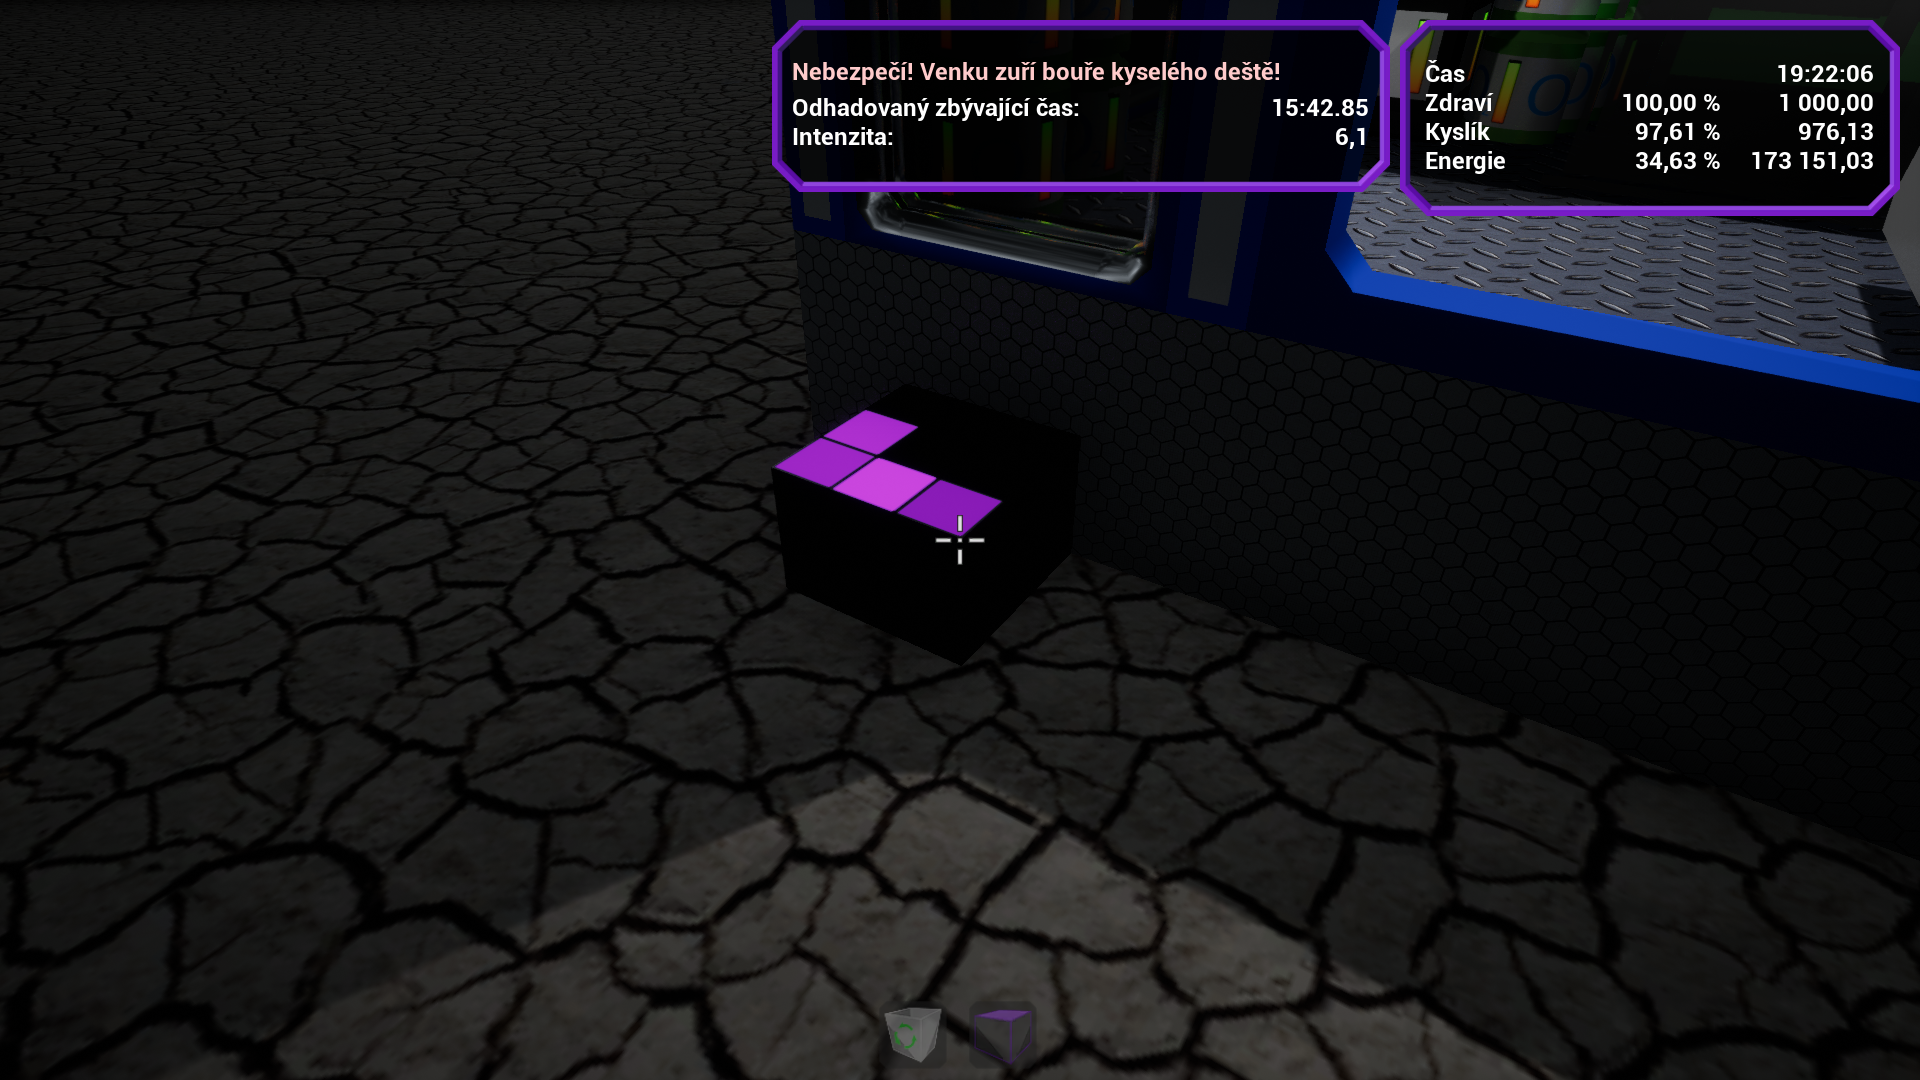
\includegraphics[ width=140mm]{../img/user/rain/4rainGeneratorAnim}

\caption{Kyselý déšť - animace zásahů}
\label{fig:user_rain_4rainGeneratorAnim}

\end{figure}


\FloatBarrier
